% =====================================================================
%  CIS 111 -- Week 7: Chapter 6 -- Arrays and Array Lists
%  LaTeX Beamer conversion of
%  cis111-w07-Arrays_and_Array_Lists-20260315.pptx
%
%  Compile with:  pdflatex cis111-w07-Arrays_and_Array_Lists.tex
%  Images are expected in ./images/
% =====================================================================
\documentclass[aspectratio=43,10pt,t]{beamer}

\usepackage[utf8]{inputenc}
\usepackage[T1]{fontenc}
\usepackage[scaled=0.92]{helvet}   % Arial-like sans (as in the original)
\usepackage{courier}               % Courier (as in the original code)
\renewcommand{\familydefault}{\sfdefault}
\usepackage{graphicx}
\usepackage{listings}
\usepackage{xcolor}
\usepackage{tikz}
\graphicspath{{images/}}

% ---------------------------------------------------------------------
%  Hidden slides
%  The Self Check slides were *hidden* in the original PowerPoint.
%  They are kept here but hidden by default.
%    \newcommand{\hiddenslides}{0}   -> hide them (like the original)
%    \newcommand{\hiddenslides}{1-}  -> show them
% ---------------------------------------------------------------------
\newcommand{\hiddenslides}{0}

% ---------------------------------------------------------------------
%  Colours
% ---------------------------------------------------------------------
\definecolor{titlerule}{HTML}{FFD966}   % yellow rule under frame titles
\definecolor{callout}{HTML}{FFE14D}     % yellow call-out boxes
\definecolor{codebg}{HTML}{DDDDDD}      % grey code background
\definecolor{syntaxteal}{HTML}{1F8C8C}  % "Syntax 6.x" headings
\definecolor{kwblue}{HTML}{1F3FA8}
\definecolor{cmtteal}{HTML}{2A8FBF}
\definecolor{strred}{HTML}{B22222}

% ---------------------------------------------------------------------
%  Beamer look
% ---------------------------------------------------------------------
\setbeamertemplate{navigation symbols}{}
\setbeamercolor{normal text}{fg=black}
\setbeamercolor{structure}{fg=black}
\setbeamercolor{frametitle}{fg=black}
\setbeamerfont{frametitle}{series=\bfseries,size=\large}
\setbeamertemplate{frametitle}{%
  \vskip2mm
  \usebeamerfont{frametitle}\insertframetitle\par
  \vskip-0.5mm
  {\color{titlerule}\rule{0.76\paperwidth}{1.3pt}}\par
}
\setbeamertemplate{itemize item}{\small$\blacksquare$}
\setbeamertemplate{itemize subitem}{\scriptsize$\blacksquare$}
\setbeamertemplate{itemize subsubitem}{\tiny$\blacksquare$}
\setbeamerfont{itemize/enumerate body}{size=\small}
\setbeamerfont{itemize/enumerate subbody}{size=\small}
\setbeamerfont{itemize/enumerate subsubbody}{size=\small}
\setbeamertemplate{footline}{%
  \hfill\color{gray}\scriptsize\insertframenumber\hspace*{4mm}\vspace*{2mm}}
\setbeamersize{text margin left=7mm,text margin right=7mm}

% ---------------------------------------------------------------------
%  Code listings (Java)
% ---------------------------------------------------------------------
\lstdefinestyle{java}{
  language=Java,
  basicstyle=\ttfamily\scriptsize,
  keywordstyle=\color{kwblue},
  commentstyle=\color{cmtteal},
  stringstyle=\color{strred},
  backgroundcolor=\color{codebg},
  frame=single, rulecolor=\color{codebg}, framesep=3pt,
  columns=fullflexible, keepspaces=true,
  showstringspaces=false, tabsize=4,
  xleftmargin=3pt, xrightmargin=3pt,
  aboveskip=4pt, belowskip=4pt,
  upquote=true,
}
\lstset{style=java}
% plain console output (yellow box)
\lstdefinestyle{output}{
  language={}, basicstyle=\ttfamily\scriptsize\color{strred},
  backgroundcolor=\color{callout}, rulecolor=\color{callout},
  commentstyle={}, keywordstyle={}, stringstyle={},
}

% full program listings (with line numbers, as in the textbook)
\definecolor{progbg}{HTML}{EDEDED}
\definecolor{lineno}{HTML}{1F5FAF}
\lstdefinestyle{program}{
  style=java,
  basicstyle=\ttfamily\fontsize{6.2}{7.2}\selectfont,
  backgroundcolor=\color{progbg}, rulecolor=\color{progbg},
  numbers=left, numberstyle=\ttfamily\bfseries\fontsize{6}{7.2}\selectfont\color{lineno},
  numbersep=6pt, xleftmargin=14pt, framexleftmargin=0pt,
  breaklines=true, breakindent=24pt, breakatwhitespace=true,
}
% "Program Run" box:  \programrun{width}{content}
\newcommand{\programrun}[2]{%
  \begin{minipage}{#1}
    {\bfseries\small\color{lineno} Program Run}\par\vskip1mm
    {\setlength{\fboxsep}{4pt}\colorbox{progbg}{%
      \parbox{\dimexpr\linewidth-8pt\relax}{\ttfamily\fontsize{6}{7.4}\selectfont #2}}}
  \end{minipage}}
\newcommand{\userinput}[1]{\textcolor{lineno}{#1}}

% ---------------------------------------------------------------------
%  Helpers
% ---------------------------------------------------------------------
\newcommand{\code}[1]{\texttt{#1}}
% yellow call-out box:  \callout[width]{text}
\newcommand{\callout}[2][\linewidth]{%
  {\setlength{\fboxsep}{3pt}\colorbox{callout}{%
    \parbox{\dimexpr#1-6pt\relax}{\raggedright\footnotesize #2}}}}
% small yellow label (replaces the arrow labels "reference"/"value")
\newcommand{\ptag}[1]{{\setlength{\fboxsep}{1.5pt}\colorbox{callout}{\scriptsize #1}}}
\newcommand{\answer}{\textbf{Answer:}\ }
\newcommand{\syntaxtitle}[2]{\textcolor{syntaxteal}{Syntax #1}\ #2}

% ---------------------------------------------------------------------
\title{Chapter 6 -- Arrays and Array Lists}
\date{}

\begin{document}

% =====================================================================
%  1  Title
% =====================================================================
\begin{frame}[plain]
  \vskip2mm
  {\Large\bfseries Chapter 6 -- Arrays and Array Lists\par}
  \vskip-0.5mm
  {\color{titlerule}\rule{0.76\paperwidth}{1.3pt}}\par
  \vfill
  \centering
  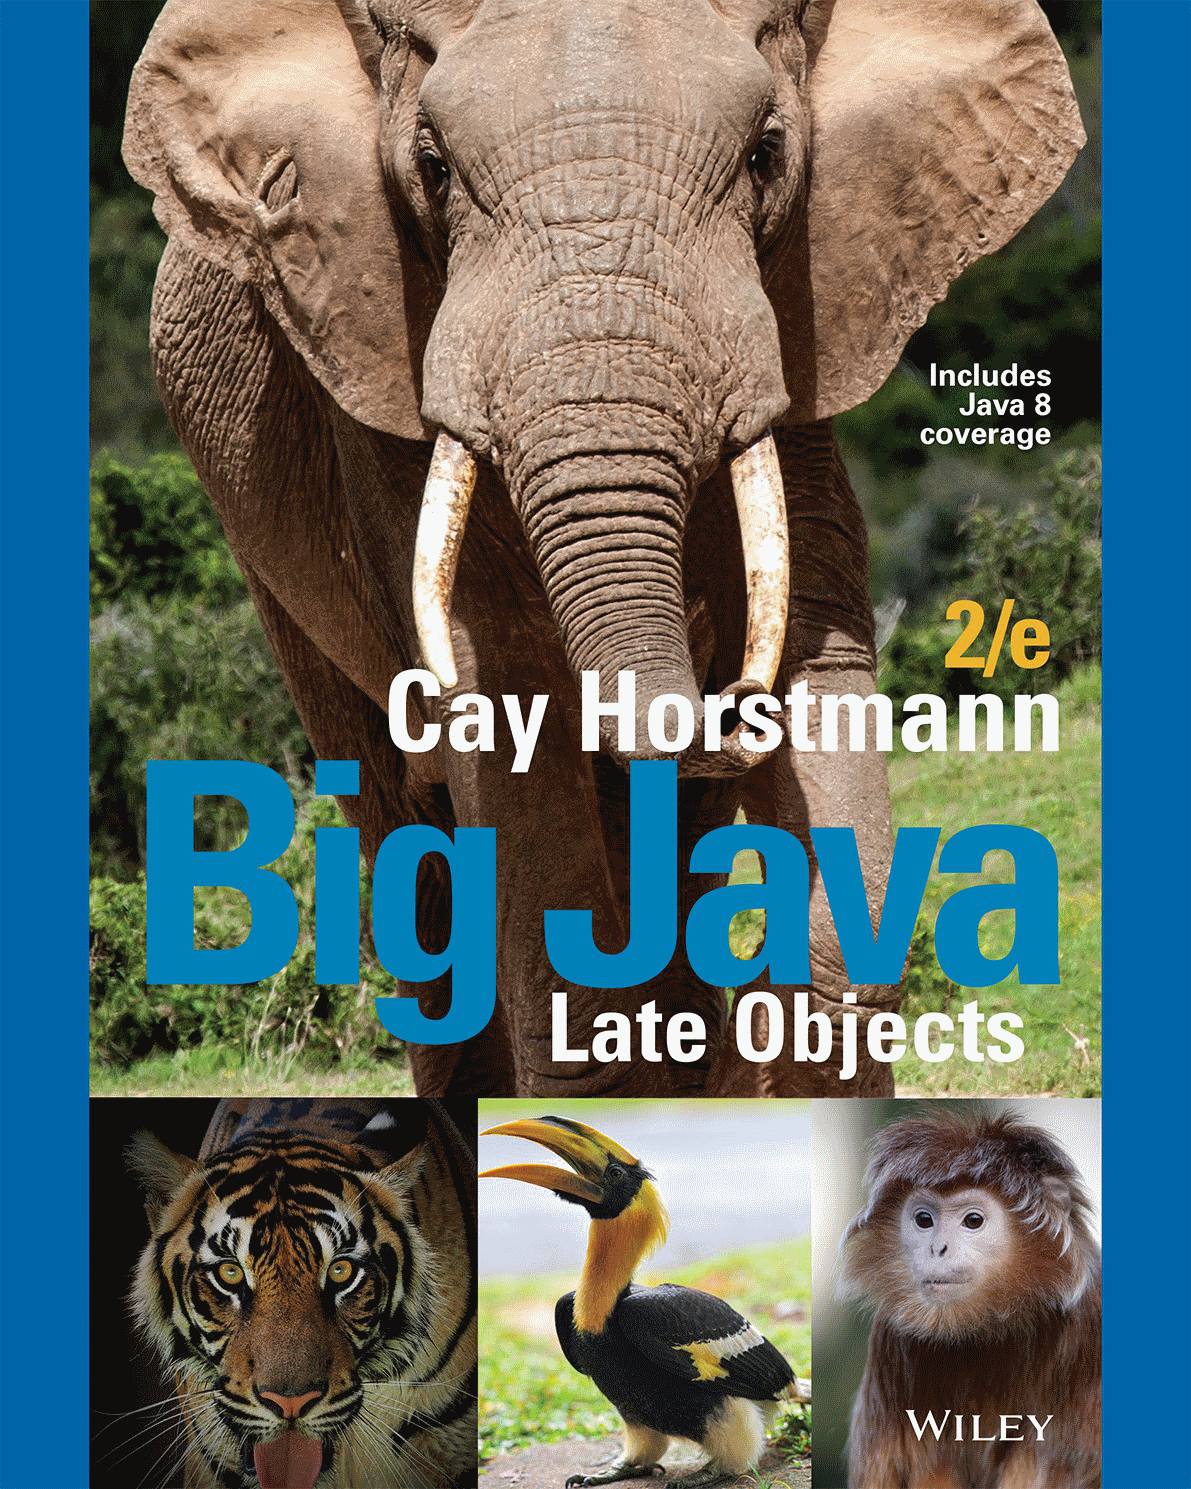
\includegraphics[height=0.78\paperheight]{image1.png}
  \vfill
\end{frame}

% =====================================================================
%  2  Chapter Goals
% =====================================================================
\begin{frame}{Chapter Goals}
  \centering
  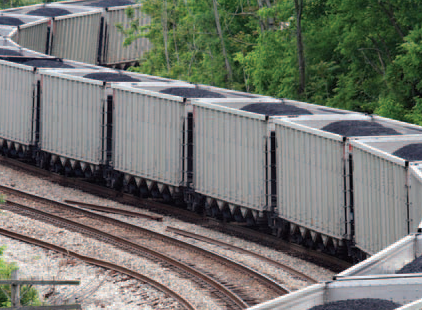
\includegraphics[width=0.5\paperwidth]{image2-cropped.png}
  \vskip3mm
  \raggedright
  \begin{itemize}
    \item To collect elements using arrays and array lists
    \item To use the enhanced for loop for traversing arrays and array lists
    \item To learn common algorithms for processing arrays and array lists
    \item To work with two-dimensional arrays
  \end{itemize}
\end{frame}

\section{Arrays}

% =====================================================================
%  3  Arrays
% =====================================================================
\begin{frame}{Arrays}
  \begin{columns}[T]
    \begin{column}{0.82\textwidth}
      \begin{itemize}
        \item A Computer Program often needs to store a list of values and then process them
        \item For example, if you had this list of values, how many variables would you need?
          \begin{itemize}
            \item \code{double input1, input2, input3\ldots.}
          \end{itemize}
        \item Arrays to the rescue!
        \item An array collects sequences of values of the same type
      \end{itemize}
    \end{column}
    \begin{column}{0.14\textwidth}
      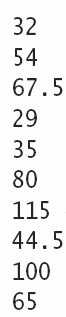
\includegraphics[height=0.62\paperheight]{image3.png}
    \end{column}
  \end{columns}
\end{frame}

% =====================================================================
%  4  Declaring an Array
% =====================================================================
\begin{frame}[fragile]{Declaring an Array}
  \begin{itemize}
    \item Declaring an array is a two step process
  \end{itemize}
\begin{lstlisting}[xleftmargin=6mm]
1)  double[] values;           // declare array variable
2)  values = new double[10];   // initialize array
\end{lstlisting}
  \centering
  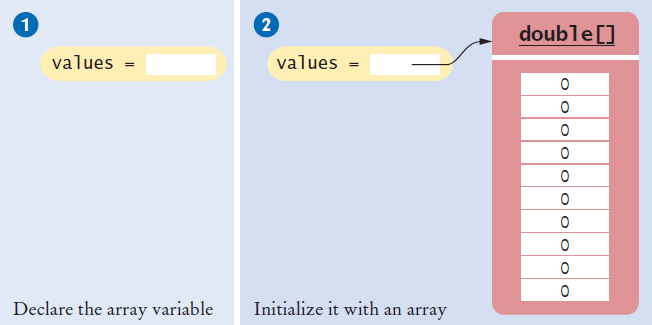
\includegraphics[width=0.72\paperwidth]{image4.png}\par
  \vskip1mm
  \callout[0.55\linewidth]{You cannot use the array until you tell the compiler the size of the array in step 2.}
\end{frame}

% =====================================================================
%  5  Declaring and Initializing an Array
% =====================================================================
\begin{frame}{Declaring and Initializing an Array}
  \begin{itemize}
    \item You can declare and set the initial contents of all elements by:
  \end{itemize}
  \vskip1mm
  \begin{center}
    \begin{tabular}{ccccc}
      \footnotesize Type & \footnotesize Braces & \footnotesize Array name &
      \footnotesize Contents list & \footnotesize Semicolon\\
      \code{int} & \code{[ ]} & \code{primes =} & \code{\{ 2, 3, 5, 7\}} & \code{;}
    \end{tabular}
  \end{center}
  \vskip1mm
  \begin{itemize}
    \item You are declaring that
      \begin{itemize}
        \item There is an array named \code{primes}
        \item The elements inside are of type \code{int}
        \item Reserve space for four elements
          \begin{itemize}
            \item The compiler counts them for you!
          \end{itemize}
        \item Set initial values to 2, 3, 5, and 7
        \item Note the curly braces around the contents list
      \end{itemize}
  \end{itemize}
\end{frame}

% =====================================================================
%  6  Accessing Array Elements
% =====================================================================
\begin{frame}[fragile]{Accessing Array Elements}
  \begin{itemize}
    \item Each element is numbered
      \begin{itemize}
        \item We call this the \emph{index}
        \item Access an element by:
          \begin{itemize}
            \item Name of the array
            \item Index number
            \item \code{values[i]}
          \end{itemize}
      \end{itemize}
  \end{itemize}
  \begin{columns}[c]
    \begin{column}{0.5\textwidth}
\begin{lstlisting}
public static void main(String[] args)
{
  double values[];
  values = new double[10];
  values[4] = 35;
}
\end{lstlisting}
    \end{column}
    \begin{column}{0.48\textwidth}
      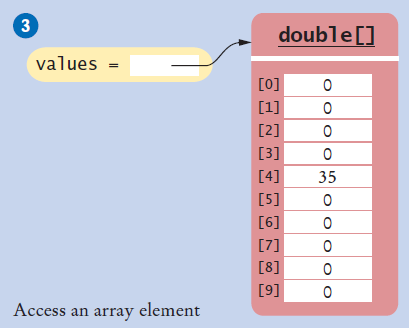
\includegraphics[width=\linewidth]{image5.png}
    \end{column}
  \end{columns}
\end{frame}

% =====================================================================
%  7  Syntax 6.1 Array
% =====================================================================
\begin{frame}{\syntaxtitle{6.1}{Array}}
  \vfill
  \centering
  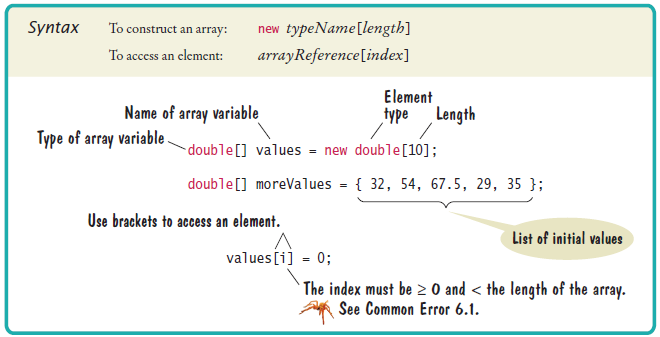
\includegraphics[width=0.86\paperwidth]{image6.png}
  \vfill
\end{frame}

% =====================================================================
%  8  Array Index Numbers
% =====================================================================
\begin{frame}[fragile]{Array Index Numbers}
  \begin{columns}[T]
    \begin{column}{0.72\textwidth}
      \begin{itemize}
        \item Array index numbers start at 0
          \begin{itemize}
            \item The rest are positive integers
          \end{itemize}
        \item A 10 element array has indices 0 through 9
          \begin{itemize}
            \item \textcolor{red}{There is NO element 10!}
          \end{itemize}
      \end{itemize}
      \vskip2mm
      \callout{The first element is at index 0 \hfill$\Rightarrow$}
\begin{lstlisting}
public static void main(String[] args)
{
  double values[];
  values = new double[10];
}
\end{lstlisting}
      \callout{The last element is at index 9 \hfill$\Rightarrow$}
    \end{column}
    \begin{column}{0.25\textwidth}
      \vskip10mm
      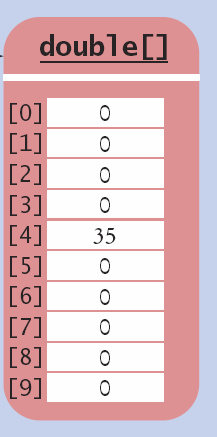
\includegraphics[width=\linewidth]{image7a-cropped.png}
    \end{column}
  \end{columns}
\end{frame}

% =====================================================================
%  9  Array Bounds Checking
% =====================================================================
\begin{frame}[fragile]{Array Bounds Checking}
  \begin{itemize}
    \item An array knows how many elements it can hold
      \begin{itemize}
        \item \code{values.length} is the size of the array named \code{values}
        \item It is an integer value (index of the last element + 1)
      \end{itemize}
    \item Use this to range check and prevent bounds errors
  \end{itemize}
\begin{lstlisting}[linewidth=0.85\linewidth,xleftmargin=6mm]
public static void main(String[] args)
{
  int i = 10, value = 34;
  double values[];
  values = new double[10];
  if (0 <= i && i < values.length)   // length is 10
  {
    values[i] = value;
  }
}
\end{lstlisting}
  \hfill
  \callout[0.5\linewidth]{Strings and arrays use different syntax to find their length:\\
    \quad Strings:\ \ \code{name.length()}\\
    \quad Arrays:\ \ \ \code{values.length}}
\end{frame}

% =====================================================================
%  10  Summary: Declaring Arrays
% =====================================================================
\begin{frame}{Summary: Declaring Arrays}
  \vfill
  \centering
  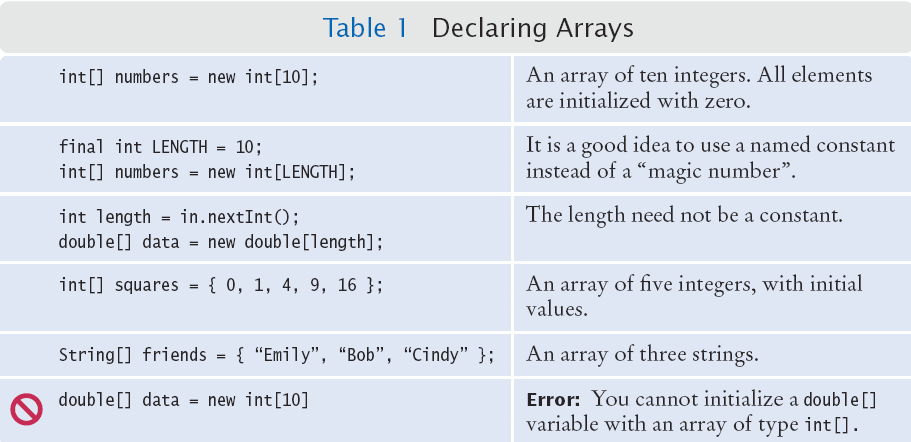
\includegraphics[width=\linewidth]{image8.png}
  \vfill
\end{frame}

% =====================================================================
%  11  Array Aliases
% =====================================================================
\begin{frame}[fragile]{Array Aliases}
  \begin{itemize}
    \item You can make one array reference refer to the same contents of another array reference:
  \end{itemize}
\begin{lstlisting}[linewidth=0.85\linewidth,xleftmargin=6mm]
int[] scores = { 10, 9, 7, 4, 5 };
int[] values = scores;  // Copying the array reference
\end{lstlisting}
  \vskip2mm
  \begin{columns}[b]
    \begin{column}{0.45\textwidth}
      \callout{An array variable specifies the location of an array. Copying the reference yields a second reference to the same array.}
    \end{column}
    \begin{column}{0.53\textwidth}
      \centering
      {\footnotesize References \hfill Array contents}\\[1mm]
      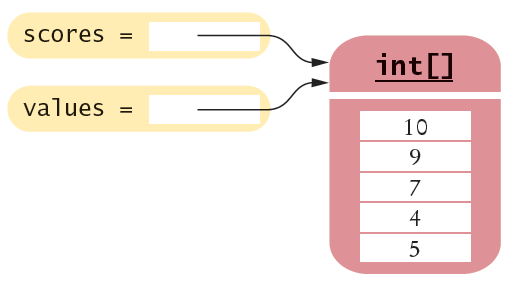
\includegraphics[width=\linewidth]{image9.png}
    \end{column}
  \end{columns}
\end{frame}

% =====================================================================
%  12--16  Self Checks 6.1--6.6   (hidden in the original)
% =====================================================================
\begin{frame}<\hiddenslides>{Self Check 6.1}
  Declare an array of integers containing the first five prime numbers.
  \vskip4mm
  \answer\code{int[] primes = \{ 2, 3, 5, 7, 11 \};}
\end{frame}

\begin{frame}<\hiddenslides>[fragile]{Self Check 6.2}
  Assume the array \code{primes} has been initialized as described in Self Check 1.
  What does it contain after executing the following loop?
\begin{lstlisting}[linewidth=0.6\linewidth,xleftmargin=8mm,backgroundcolor={},frame=none]
for (int i = 0; i < 2; i++)
{
   primes[4 - i] = primes[i];
}
\end{lstlisting}
  \answer\code{2, 3, 5, 3, 2}
\end{frame}

\begin{frame}<\hiddenslides>[fragile]{Self Check 6.3}
  Assume the array \code{primes} has been initialized as described in Self Check 1.
  What does it contain after executing the following loop?
\begin{lstlisting}[linewidth=0.6\linewidth,xleftmargin=8mm,backgroundcolor={},frame=none]
for (int i = 0; i < 5; i++)
{
   primes[i]++;
}
\end{lstlisting}
  \answer\code{3, 4, 6, 8, 12}
\end{frame}

\begin{frame}<\hiddenslides>{Self Check 6.5}
  Declare an array called \code{words} that can hold ten elements of type \code{String}.
  \vskip4mm
  \answer\code{String[] words = new String[10];}
\end{frame}

\begin{frame}<\hiddenslides>{Self Check 6.6}
  Declare an array containing two strings, "\code{Yes}", and "\code{No}".
  \vskip4mm
  \answer\code{String[] words = \{ "Yes", "No" \};}
\end{frame}

% =====================================================================
%  17  Common Error -- Array Bounds Errors
% =====================================================================
\begin{frame}[fragile]{Common Error}
  \begin{columns}[T]
    \begin{column}{0.74\textwidth}
      \begin{itemize}
        \item Array Bounds Errors
          \begin{itemize}
            \item Accessing a nonexistent element is very common error
            \item Array indexing starts at 0
            \item Your program will abnormally end at run time
          \end{itemize}
      \end{itemize}
\begin{lstlisting}
public class OutOfBounds
{
  public static void main(String[] args)
  {
    double values[];
    values = new double[10];
    values[10] = 100;
  }
}
\end{lstlisting}
      \hfill\callout[0.55\linewidth]{There is no element 10: \hfill$\Rightarrow$}
    \end{column}
    \begin{column}{0.22\textwidth}
      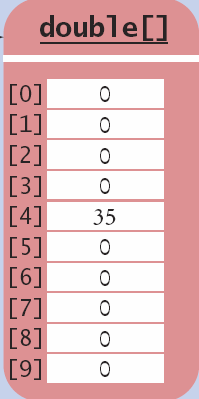
\includegraphics[width=\linewidth]{image7b-cropped.png}
    \end{column}
  \end{columns}
  \vskip2mm
\begin{lstlisting}[style=output,linewidth=0.8\linewidth,xleftmargin=10mm]
java.lang.ArrayIndexOutOfBoundsException: 10
    at OutOfBounds.main(OutOfBounds.java:7)
\end{lstlisting}
\end{frame}

% =====================================================================
%  18  Common Error -- Uninitialized Arrays
% =====================================================================
\begin{frame}[fragile]{Common Error}
  \begin{itemize}
    \item Uninitialized Arrays
      \begin{itemize}
        \item Don't forget to initialize the array variable!
        \item The compiler will catch this error
      \end{itemize}
  \end{itemize}
  \begin{columns}[c]
    \begin{column}{0.72\textwidth}
\begin{lstlisting}
double[] values;
...
values[0] = 29.95; // Error-values not initialized
\end{lstlisting}
\begin{lstlisting}[style=output]
Error: D:\Java\Unitialized.java:7:
variable values might not have been initialized
\end{lstlisting}
    \end{column}
    \begin{column}{0.26\textwidth}
      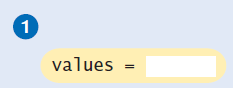
\includegraphics[width=\linewidth]{image10-cropped.png}
    \end{column}
  \end{columns}
  \vskip2mm
  \begin{columns}[c]
    \begin{column}{0.46\textwidth}
\begin{lstlisting}
double[] values;
values = new double[10];
values[0] = 29.95; // No error
\end{lstlisting}
    \end{column}
    \begin{column}{0.52\textwidth}
      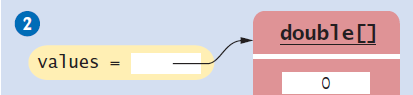
\includegraphics[width=\linewidth]{image11.png}
    \end{column}
  \end{columns}
\end{frame}

\section{The Enhanced for Loop}

% =====================================================================
%  19  The Enhanced for Loop
% =====================================================================
\begin{frame}[fragile]{The Enhanced \texttt{for} Loop}
  \begin{columns}[T]
    \begin{column}{0.56\textwidth}
      \begin{itemize}
        \item Using \code{for} loops to `walk' arrays is very common
          \begin{itemize}
            \item The enhanced \code{for} loop simplifies the process
            \item Also called the ``for each'' loop
            \item Read this code as:
              \begin{itemize}
                \item ``For each element in the array''
              \end{itemize}
          \end{itemize}
        \item As the loop proceeds, it will:
          \begin{itemize}
            \item Access each element in order (0 to length-1)
            \item Copy it to the \code{element} variable
            \item Execute loop body
          \end{itemize}
        \item Not possible to:
          \begin{itemize}
            \item Change elements
            \item Get bounds error
          \end{itemize}
      \end{itemize}
    \end{column}
    \begin{column}{0.42\textwidth}
      \vskip32mm
\begin{lstlisting}
double[] values = . . .;
double total = 0;
for (double element : values)
{
  total = total + element;
}
\end{lstlisting}
    \end{column}
  \end{columns}
\end{frame}

% =====================================================================
%  20  Syntax 6.2 The Enhanced for loop
% =====================================================================
\begin{frame}{\syntaxtitle{6.2}{The Enhanced \texttt{for} loop}}
  \vfill
  \centering
  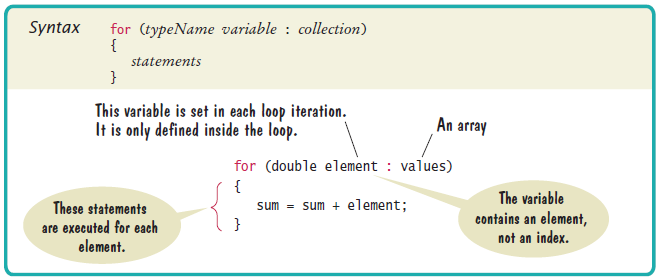
\includegraphics[width=0.86\paperwidth]{image12.png}
  \vfill
\end{frame}

% =====================================================================
%  21--22  Self Checks 6.9--6.10   (hidden in the original)
% =====================================================================
\begin{frame}<\hiddenslides>[fragile]{Self Check 6.9}
  Write an enhanced \code{for} loop that prints all elements in the array \code{values}.
  \vskip3mm
  \answer
\begin{lstlisting}[linewidth=0.6\linewidth,xleftmargin=8mm,backgroundcolor={},frame=none]
for (double x : values)
{
   System.out.println(x);
}
\end{lstlisting}
\end{frame}

\begin{frame}<\hiddenslides>[fragile]{Self Check 6.10}
  Write an enhanced \code{for} loop that multiplies all elements in a \code{double[]}
  array named \code{factors}, accumulating the result in a variable named \code{product}.
  \vskip3mm
  \answer
\begin{lstlisting}[linewidth=0.6\linewidth,xleftmargin=8mm,backgroundcolor={},frame=none]
double product = 1;
for (double f : factors)
{
   product = product * f;
}
\end{lstlisting}
\end{frame}

\section{Common Array Algorithms}

% =====================================================================
%  23  Common Array Algorithms
% =====================================================================
\begin{frame}{Common Array Algorithms}
  \begin{itemize}
    \item Filling an Array
    \item Sum and Average Values
    \item Find the Maximum or Minimum
    \item Output Elements with Separators
    \item Linear Search
    \item Removing an Element
    \item Inserting an Element
    \item Swapping Elements
    \item Copying Arrays
    \item Reading Input
  \end{itemize}
\end{frame}

% =====================================================================
%  24  Common Algorithms 1 and 2
% =====================================================================
\begin{frame}[fragile]{Common Algorithms 1 and 2}
  1) Filling an Array
  \begin{itemize}
    \item Initialize an array to a set of calculated values
    \item Example:\ \ Fill an array with squares of 0 through 10
  \end{itemize}
\begin{lstlisting}[linewidth=0.62\linewidth,xleftmargin=0.2\linewidth]
int[] values = new int[11];
for (int i = 0; i < values.length; i++)
{
  values[i] = i * i;
}
\end{lstlisting}
  \vskip2mm
  2) Sum and Average
  \begin{itemize}
    \item Use enhanced \code{for} loop, and make sure not to divide by zero
  \end{itemize}
\begin{lstlisting}[linewidth=0.8\linewidth,xleftmargin=0.08\linewidth]
double total = 0, average = 0;
for (double element : values)
{
  total = total + element;
}
if (values.length > 0) {
  average = total / values.length;
}
\end{lstlisting}
\end{frame}

% =====================================================================
%  25  Common Algorithms 3
% =====================================================================
\begin{frame}[fragile]{Common Algorithms 3}
  \begin{itemize}
    \item Maximum and Minimum
      \begin{itemize}
        \item Set largest to first element
        \item Use for or enhanced for loop
        \item Use the same logic for minimum
      \end{itemize}
  \end{itemize}
  \begin{columns}[c]
    \begin{column}{0.6\textwidth}
\begin{lstlisting}
double largest = values[0];
for (int i = 1; i < values.length; i++)
{
  if (values[i] > largest)
  {
    largest = values[i];
  }
}
\end{lstlisting}
    \end{column}
    \begin{column}{0.38\textwidth}
      \callout{Typical \code{for} loop to find maximum}
    \end{column}
  \end{columns}
  \begin{columns}[T]
    \begin{column}{0.48\textwidth}
\begin{lstlisting}
double largest = values[0];
for (double element : values)
{
  if (element > largest)
    largest = element;
}
\end{lstlisting}
      \callout{Enhanced \code{for} to find maximum}
    \end{column}
    \begin{column}{0.48\textwidth}
\begin{lstlisting}
double smallest = values[0];
for (double element : values)
{
  if (element < smallest)
    smallest = element;
}
\end{lstlisting}
      \callout{Enhanced \code{for} to find minimum}
    \end{column}
  \end{columns}
\end{frame}

% =====================================================================
%  26  Common Algorithms 4
% =====================================================================
\begin{frame}[fragile]{Common Algorithms 4}
  \begin{itemize}
    \item Element Separators
      \begin{itemize}
        \item Output all elements with separators between them
        \item No separator before the first or after the last element
      \end{itemize}
  \end{itemize}
  \begin{columns}[c]
    \begin{column}{0.58\textwidth}
\begin{lstlisting}
for (int i = 0; i < values.length; i++)
{
  if (i > 0)
  {
    System.out.print(" | ");
  }
  System.out.print(values[i]);
}
\end{lstlisting}
    \end{column}
    \begin{column}{0.38\textwidth}
      {\setlength{\fboxsep}{3pt}\colorbox{progbg}{\ttfamily\footnotesize 32 | 54 | 67.5 | 29 | 35}}
    \end{column}
  \end{columns}
  \begin{itemize}
    \item Handy Array method:\ \ \textbf{\code{Arrays.toString}}\code{()}
      \begin{itemize}
        \item Useful for debugging!
      \end{itemize}
  \end{itemize}
  \hfill{\setlength{\fboxsep}{3pt}\colorbox{progbg}{\ttfamily\footnotesize [32, 54, 67.5, 29, 35]}}\hspace*{6mm}
\begin{lstlisting}[linewidth=0.7\linewidth,xleftmargin=0.12\linewidth]
import java.util.*;
System.out.println(Arrays.toString(values));
\end{lstlisting}
\end{frame}

% =====================================================================
%  27  Common Algorithms 5 -- Linear Search
% =====================================================================
\begin{frame}[fragile]{Common Algorithms 5}
  \begin{itemize}
    \item Linear Search
      \begin{itemize}
        \item Search for a specific value in an array
        \item Start from the beginning (left), stop if/when it is found
        \item Uses a boolean \code{found} flag to stop loop if found
      \end{itemize}
  \end{itemize}
  \begin{columns}[T]
    \begin{column}{0.66\textwidth}
\begin{lstlisting}[basicstyle=\ttfamily\fontsize{6.2}{7.1}\selectfont]
int searchedValue = 100;  int pos = 0;
boolean found = false;
while (pos < values.length && !found)
{
  if (values[pos] == searchedValue)
  {
    found = true;
  }
  else
  {
    pos++;
  }
}
if (found)
{
  System.out.println("Found at position: " + pos);
}
else
{
  System.out.println("Not found");
}
\end{lstlisting}
    \end{column}
    \begin{column}{0.32\textwidth}
      \vskip10mm
      \callout{Compound condition to prevent bounds error if value not found.}
    \end{column}
  \end{columns}
\end{frame}

% =====================================================================
%  28  Common Algorithms 6a -- Removing (unordered)
% =====================================================================
\begin{frame}[fragile]{Common Algorithms 6a}
  \begin{itemize}
    \item Removing an element (at a given position)
      \begin{itemize}
        \item Requires tracking the `current size' (\# of valid elements)
        \item But don't leave a `hole' in the array!
        \item Solution depends on if you have to maintain `order'
          \begin{itemize}
            \item If not, find the last valid element, copy over position, update size
          \end{itemize}
      \end{itemize}
  \end{itemize}
  \begin{columns}[T]
    \begin{column}{0.38\textwidth}
      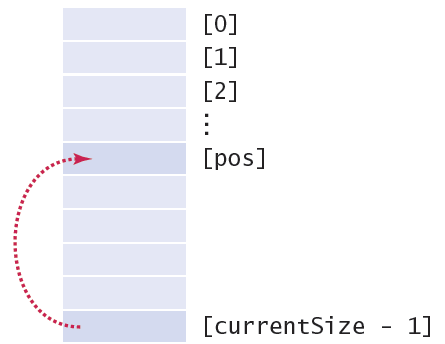
\includegraphics[width=\linewidth]{image15-cropped.png}
    \end{column}
    \begin{column}{0.6\textwidth}
      \vskip4mm
\begin{lstlisting}
values[pos] = values[currentSize - 1];
currentSize--;
\end{lstlisting}
    \end{column}
  \end{columns}
\end{frame}

% =====================================================================
%  29  Common Algorithms 6b -- Removing (ordered)
% =====================================================================
\begin{frame}[fragile]{Common Algorithms 6b}
  \begin{itemize}
    \item Removing an element and maintaining order
      \begin{itemize}
        \item Requires tracking the `current size' (\# of valid elements)
        \item But don't leave a `hole' in the array!
        \item Solution depends on if you have to maintain `order'
          \begin{itemize}
            \item If so, move all of the valid elements after \code{pos} up one spot, update size
          \end{itemize}
      \end{itemize}
  \end{itemize}
  \begin{columns}[T]
    \begin{column}{0.38\textwidth}
      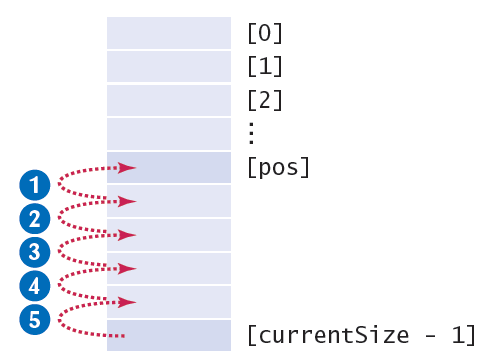
\includegraphics[width=\linewidth]{image16.png}
    \end{column}
    \begin{column}{0.6\textwidth}
      \vskip6mm
\begin{lstlisting}
for (int i = pos; i < currentSize - 1; i++)
{
  values[i] = values[i + 1];
}
currentSize--;
\end{lstlisting}
    \end{column}
  \end{columns}
\end{frame}

% =====================================================================
%  30  Common Algorithms 7 -- Inserting (unordered)
% =====================================================================
\begin{frame}[fragile]{Common Algorithms 7}
  \begin{itemize}
    \item Inserting an Element
      \begin{itemize}
        \item Solution depends on if you have to maintain `order'
          \begin{itemize}
            \item If not, just add it to the end and update the size
          \end{itemize}
      \end{itemize}
  \end{itemize}
  \begin{columns}[T]
    \begin{column}{0.38\textwidth}
      \vskip14mm
      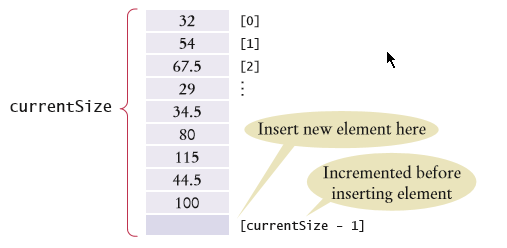
\includegraphics[width=\linewidth]{image17.png}
    \end{column}
    \begin{column}{0.6\textwidth}
\begin{lstlisting}
if (currentSize < values.length)
{
  currentSize++;
  values[currentSize - 1] = newElement;
}
\end{lstlisting}
    \end{column}
  \end{columns}
\end{frame}

% =====================================================================
%  31  Common Algorithms 7 -- Inserting (ordered)
% =====================================================================
\begin{frame}[fragile]{Common Algorithms 7}
  \begin{itemize}
    \item Inserting an Element
      \begin{itemize}
        \item Solution depends on if you have to maintain `order'
          \begin{itemize}
            \item If so, find the right spot for the new element, move all of the valid
                  elements after `pos' down one spot, insert the new element, and update size
          \end{itemize}
      \end{itemize}
  \end{itemize}
  \begin{columns}[T]
    \begin{column}{0.32\textwidth}
      \vskip8mm
      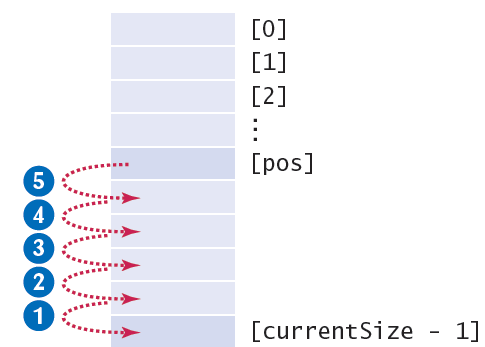
\includegraphics[width=\linewidth]{image18.png}
    \end{column}
    \begin{column}{0.66\textwidth}
\begin{lstlisting}
if (currentSize < values.length)
{
  currentSize++;
  for (int i = currentSize - 1; i > pos; i--)
  {
    values[i] = values[i - 1];  // move down
  }
  values[pos] = newElement;     // fill hole
}
\end{lstlisting}
    \end{column}
  \end{columns}
\end{frame}

% =====================================================================
%  32  Common Algorithms 8 -- Swapping
% =====================================================================
\begin{frame}[fragile]{Common Algorithms 8}
  \begin{itemize}
    \item Swapping Elements
      \begin{itemize}
        \item Three steps using a temporary variable
      \end{itemize}
  \end{itemize}
  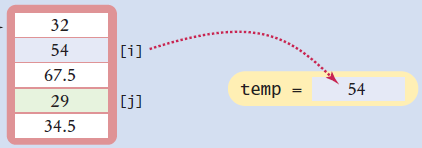
\includegraphics[width=0.44\paperwidth]{image19.png}\par
  \hspace*{0.2\paperwidth}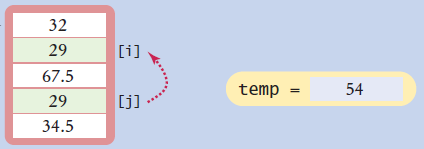
\includegraphics[width=0.44\paperwidth]{image20.png}\par
  \begin{minipage}[b]{0.4\linewidth}
\begin{lstlisting}
double temp = values[i];
values[i] = values[j];
values[j] = temp;
\end{lstlisting}
  \end{minipage}\hfill
  \begin{minipage}[b]{0.52\linewidth}
    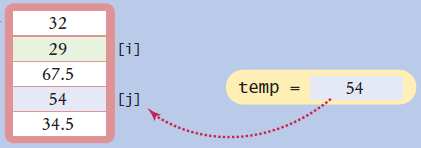
\includegraphics[width=\linewidth]{image21.png}
  \end{minipage}
\end{frame}

% =====================================================================
%  33  Common Algorithms 9a -- Copying Arrays
% =====================================================================
\begin{frame}[fragile]{Common Algorithms 9a}
  \begin{columns}[T]
    \begin{column}{0.6\textwidth}
      \begin{itemize}
        \item Copying Arrays
          \begin{itemize}
            \item Not the same as copying only the reference
              \begin{itemize}
                \item Copying creates two sets of contents!
              \end{itemize}
            \item Use the \code{Arrays.copyOf} method
          \end{itemize}
      \end{itemize}
    \end{column}
    \begin{column}{0.38\textwidth}
      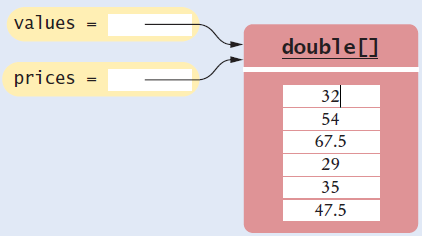
\includegraphics[width=\linewidth]{image22.png}
    \end{column}
  \end{columns}
\begin{lstlisting}[linewidth=0.9\linewidth,xleftmargin=0.03\linewidth]
double[] values = new double[6];
. . . // Fill array
double[] prices = values;   // Only a reference so far
prices = Arrays.copyOf(values, values.length);
// copyOf creates the new copy, returns a reference
\end{lstlisting}
  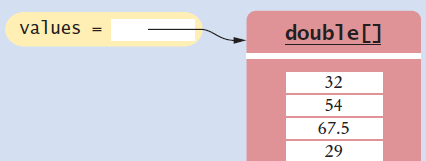
\includegraphics[width=0.46\linewidth]{image23-cropped.png}\hfill
  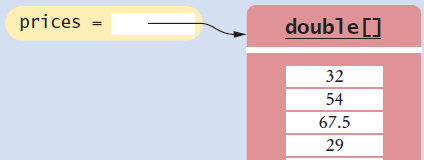
\includegraphics[width=0.46\linewidth]{image24-cropped.png}
\end{frame}

% =====================================================================
%  34  Common Algorithms 9b -- Growing an Array
% =====================================================================
\begin{frame}[fragile]{Common Algorithms 9b}
  \begin{itemize}
    \item Growing an array
      \begin{itemize}
        \item Copy the contents of one array to a larger one
        \item Change the reference of the original to the larger one
      \end{itemize}
    \item Example:\ \ Double the size of an existing array
      \begin{itemize}
        \item Use the \code{Arrays.copyOf} method
        \item Use \code{2 *} in the second parameter
      \end{itemize}
  \end{itemize}
\begin{lstlisting}
double[] values = new double[6];
. . . // Fill array
double[] newValues = Arrays.copyOf(values, 2 * values.length);
values = newValues;
\end{lstlisting}
  \hfill\callout[0.45\linewidth]{\code{Arrays.copyOf} second parameter is the length of the new array}
\end{frame}

% =====================================================================
%  35  Common Algorithms 10 -- Reading Input
% =====================================================================
\begin{frame}[fragile]{Common Algorithms 10}
  \begin{itemize}
    \item Reading Input
      \begin{itemize}
        \item A:\ \ Known number of values to expect
          \begin{itemize}
            \item Make an array that size and fill it one-by-one
          \end{itemize}
      \end{itemize}
  \end{itemize}
\begin{lstlisting}[linewidth=0.85\linewidth,xleftmargin=0.12\linewidth]
double[] inputs = new double[NUMBER_OF_INPUTS];
for (int i = 0; i < inputs.length; i++)
{
  inputs[i] = in.nextDouble();
}
\end{lstlisting}
  \begin{itemize}
    \item[]
      \begin{itemize}
        \item B: Unknown number of values
          \begin{itemize}
            \item Make maximum sized array, maintain as partially filled array
          \end{itemize}
      \end{itemize}
  \end{itemize}
\begin{lstlisting}[linewidth=0.88\linewidth,xleftmargin=0.1\linewidth]
double[] inputs = new double[MAX_INPUTS];
int currentSize = 0;
while (in.hasNextDouble() && currentSize < inputs.length)
{
  inputs[currentSize] = in.nextDouble();
  currentSize++;
}
\end{lstlisting}
\end{frame}

% =====================================================================
%  36  LargestInArray.java (1)
% =====================================================================
\begin{frame}[fragile]{LargestInArray.java (1)}
\begin{lstlisting}[style=program]
import java.util.Scanner;

/**
   This program reads a sequence of values and prints them, marking the largest value.
*/
public class LargestInArray
{
   public static void main(String[] args)
   {
      final int LENGTH = 100;
      double[] data = new double[LENGTH];
      int currentSize = 0;

      // Read inputs

      System.out.println("Please enter values, Q to quit:");
      Scanner in = new Scanner(System.in);
      while (in.hasNextDouble() && currentSize < data.length)
      {
         data[currentSize] = in.nextDouble();
         currentSize++;
      }
\end{lstlisting}
  \begin{tikzpicture}[remember picture,overlay]
    \node[anchor=south east] at ([xshift=-8mm,yshift=10mm]current page.south east)
      {\callout[0.3\paperwidth]{Input values and store in next available index of the array}};
  \end{tikzpicture}
\end{frame}

% =====================================================================
%  37  LargestInArray.java (2)
% =====================================================================
\begin{frame}[fragile]{LargestInArray.java (2)}
  \begin{columns}[T]
    \begin{column}{0.62\textwidth}
\begin{lstlisting}[style=program,firstnumber=24,basicstyle=\ttfamily\fontsize{5.9}{7}\selectfont]
      // Find the largest value

      double largest = data[0];
      for (int i = 1; i < currentSize; i++)
      {
         if (data[i] > largest)
         {
            largest = data[i];
         }
      }

      // Print all values, marking the largest

      for (int i = 0; i < currentSize; i++)
      {
         System.out.print(data[i]);
         if (data[i] == largest)
         {
            System.out.print(" <== largest value");
         }
         System.out.println();
      }
   }
}
\end{lstlisting}
    \end{column}
    \begin{column}{0.37\textwidth}
      \vskip4mm
      \callout{Use a \code{for} loop and the `Find the largest' algorithm}
      \vskip8mm
      \programrun{\linewidth}{%
        \fontsize{5.7}{7}\selectfont
        Please enter values, Q to quit:\\
        \userinput{35 80 115 44.5 Q}\\
        35\\
        80\\
        115 <== largest value\\
        44.5}
    \end{column}
  \end{columns}
\end{frame}

% =====================================================================
%  38  Special Topic: Sorting Arrays
% =====================================================================
\begin{frame}[fragile]{Special Topic:\ \ Sorting Arrays}
  \begin{itemize}
    \item When you store values into an array, you can choose to either:
      \begin{itemize}
        \item Keep them unsorted (random order)
          \hfill\raisebox{-0.8\height}{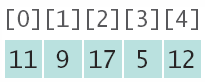
\includegraphics[width=0.2\paperwidth]{image29.png}}
        \item Sort them (Ascending or Descending\ldots)
          \hfill\raisebox{-0.8\height}{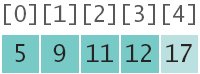
\includegraphics[width=0.2\paperwidth]{image30.png}}
      \end{itemize}
    \item A sorted array makes it much easier to find a specific value in a large data set
    \item The Java API provides an efficient sort method:
  \end{itemize}
\begin{lstlisting}
Arrays.sort(values);      // Sort all of the array
Arrays.sort(values, 0, currentSize);  // partially filled
\end{lstlisting}
\end{frame}

% =====================================================================
%  39  Special Topic: Searching
% =====================================================================
\begin{frame}{Special Topic: Searching}
  \begin{itemize}
    \item We have seen the Linear Search (6.3.5)
      \begin{itemize}
        \item It works on an array that is sorted, or unsorted
        \item Visit each element (start to end), and stop if you find a match or find the end of the array
      \end{itemize}
    \item Binary Search
      \begin{itemize}
        \item Only works for a sorted array
        \item Compare the middle element to our target
          \begin{itemize}
            \item If it is lower, exclude the lower half
            \item If it is higher, exclude the higher half
          \end{itemize}
        \item Do it again until you find the target or you cannot split what is left
      \end{itemize}
  \end{itemize}
\end{frame}

% =====================================================================
%  40  Binary Search
% =====================================================================
\begin{frame}{Binary Search}
  \begin{columns}[T]
    \begin{column}{0.64\textwidth}
      \begin{itemize}
        \item Binary Search
          \begin{itemize}
            \item Only works for a sorted array
            \item Compare the middle element to our target
              \begin{itemize}
                \item If it is lower, exclude the lower half
                \item If it is higher, exclude the higher half
                \item Do it again until you find the target or you cannot split what is left
              \end{itemize}
            \item Example:\ \ Find the value 15
          \end{itemize}
      \end{itemize}
    \end{column}
    \begin{column}{0.34\textwidth}
      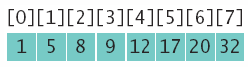
\includegraphics[width=\linewidth]{image31.png}
    \end{column}
  \end{columns}
  \vskip3mm
  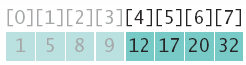
\includegraphics[width=0.29\paperwidth]{image32.png}\par
  \hspace*{0.31\paperwidth}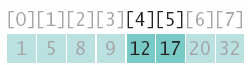
\includegraphics[width=0.29\paperwidth]{image33.png}\par
  \begin{minipage}[b]{0.66\linewidth}
    \hspace*{6mm}\footnotesize\code{Sorry, 15 is not in this array.}
  \end{minipage}\hfill
  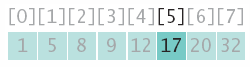
\includegraphics[width=0.29\paperwidth]{image34.png}
\end{frame}

% =====================================================================
%  41  Binary Search Example
% =====================================================================
\begin{frame}[fragile]{Binary Search Example}
\begin{lstlisting}[basicstyle=\ttfamily\scriptsize]
boolean found = false; int low = 0; int pos = 0;
int high = values.length - 1;
while (low <= high && !found)
{
  pos = (low + high) / 2;  // Midpoint of the subsequence
  if (values[pos] == searchedValue)
    { found = true; }      // Found it!
  else if (values[pos] < searchedValue)
    { low = pos + 1; }     // Look in second half
  else { high = pos - 1; } // Look in first half
}
if (found)
 { System.out.println("Found at position " + pos); }
else
 { System.out.println("Not found. Insert before position " + pos); }
\end{lstlisting}
  \vskip2mm
  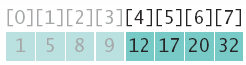
\includegraphics[width=0.3\linewidth]{image32.png}\hfill
  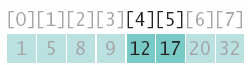
\includegraphics[width=0.3\linewidth]{image33.png}\hfill
  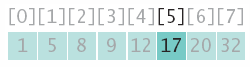
\includegraphics[width=0.3\linewidth]{image34.png}
\end{frame}

\section{Using Arrays with Methods}

% =====================================================================
%  42  Using Arrays with Methods
% =====================================================================
\begin{frame}[fragile]{Using Arrays with Methods}
  \begin{itemize}
    \item Methods can be declared to receive references as parameter variables
    \item What if we wanted to write a method to sum all of the elements in an array?
      \begin{itemize}
        \item Pass the array \emph{reference} as an argument!
      \end{itemize}
  \end{itemize}
  \begin{columns}[T]
    \begin{column}{0.56\textwidth}
      \vskip3mm
\begin{lstlisting}[linewidth=0.75\linewidth,xleftmargin=0.25\linewidth]
priceTotal = sum(prices);
\end{lstlisting}
      \hspace*{0.62\linewidth}\ptag{$\downarrow$ reference}
\begin{lstlisting}
public static double sum(double[] values)
{
  double total = 0;
  for (double element : values)
    total = total + element;
  return total;
}
\end{lstlisting}
    \end{column}
    \begin{column}{0.42\textwidth}
      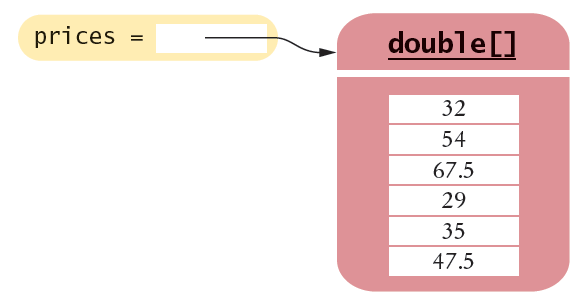
\includegraphics[width=\linewidth]{image35-cropped.png}
      \vskip6mm
      \callout{Arrays can be used as method arguments and method return values.}
    \end{column}
  \end{columns}
\end{frame}

% =====================================================================
%  43  Passing References (Step 1)
% =====================================================================
\begin{frame}[fragile]{Passing References (Step 1)}
  \begin{itemize}
    \item Passing a reference gives the called method access to all of the data elements
      \begin{itemize}
        \item It CAN change the values!
      \end{itemize}
    \item Example:\ \ Multiply each element in the passed array by the value passed in the second parameter
  \end{itemize}
  \vskip2mm
  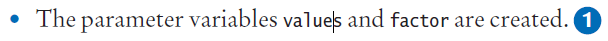
\includegraphics[width=0.73\paperwidth]{image36.png}
  \vskip3mm
\begin{lstlisting}[linewidth=0.5\linewidth,xleftmargin=0.4\linewidth]
multiply(values,       10);
\end{lstlisting}
  \hspace*{0.46\linewidth}\ptag{reference $\downarrow$}\hspace*{0.08\linewidth}\ptag{value $\downarrow$}
\begin{lstlisting}
public static void multiply(double[] data, double factor)
{
  for (int i = 0; i < data.length; i++)
    data[i] = data[i] * factor;
}
\end{lstlisting}
\end{frame}

% =====================================================================
%  44  Passing References (Step 2)
% =====================================================================
\begin{frame}{Passing References (Step 2)}
  \centering
  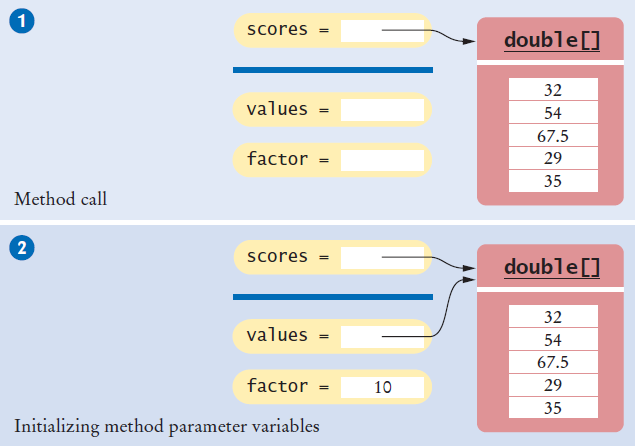
\includegraphics[height=0.66\paperheight]{image37.png}\par
  \vskip1mm
  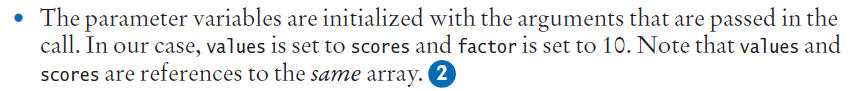
\includegraphics[width=0.81\paperwidth]{image38.png}
\end{frame}

% =====================================================================
%  45  Passing References (Steps 3 & 4)
% =====================================================================
\begin{frame}{Passing References (Steps 3 \& 4)}
  \centering
  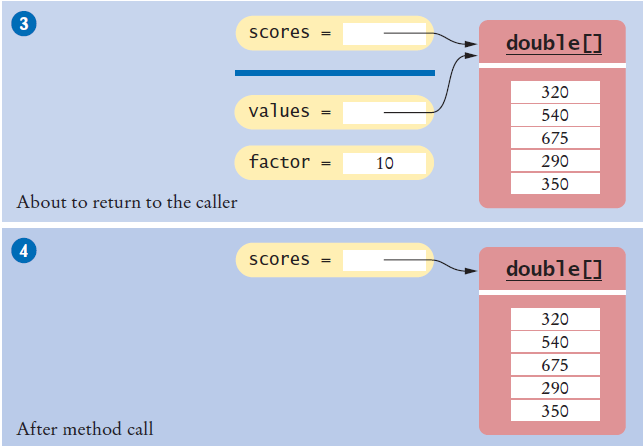
\includegraphics[height=0.64\paperheight]{image39.png}\par
  \vskip1mm
  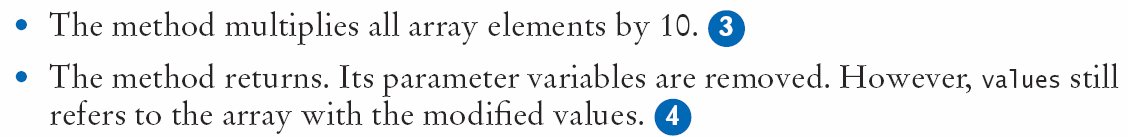
\includegraphics[width=0.81\paperwidth]{image40.png}
\end{frame}

% =====================================================================
%  46  Method Returning an Array
% =====================================================================
\begin{frame}[fragile]{Method Returning an Array}
  \begin{itemize}
    \item Methods can be declared to return an array
  \end{itemize}
\begin{lstlisting}[linewidth=0.55\linewidth,xleftmargin=0.08\linewidth]
public static int[] squares(int n)
\end{lstlisting}
  \begin{itemize}
    \item To Call: Create a compatible array reference:
  \end{itemize}
\begin{lstlisting}[linewidth=0.5\linewidth,xleftmargin=0.3\linewidth]
int[] numbers = squares(10);
\end{lstlisting}
  \begin{itemize}
    \item[]
      \begin{itemize}
        \item Call the method \hfill\ptag{value $\uparrow$}\hspace*{0.2\linewidth}
      \end{itemize}
  \end{itemize}
  \begin{columns}[c]
    \begin{column}{0.2\textwidth}
      \raggedleft\ptag{reference $\uparrow$}
    \end{column}
    \begin{column}{0.66\textwidth}
\begin{lstlisting}
public static int[] squares(int n)
{
  int[] result = new int[n];
  for (int i = 0; i < n; i++)
  {
    result[i] = i * i;
  }
  return result;
}
\end{lstlisting}
    \end{column}
    \begin{column}{0.12\textwidth}
    \end{column}
  \end{columns}
\end{frame}

% =====================================================================
%  47  Self Check 6.22   (hidden in the original)
% =====================================================================
\begin{frame}<\hiddenslides>[fragile]{Self Check 6.22}
  Consider the following method that reverses an array:
\begin{lstlisting}[linewidth=0.8\linewidth,xleftmargin=8mm,backgroundcolor={},frame=none]
public static int[] reverse(int[] values)
{
   int[] result = new int[values.length];
   for (int i = 0; i < values.length; i++)
   {
      result[i] = values[values.length - 1 - i];
   }
   return result;
}
\end{lstlisting}
  Suppose the \code{reverse} method is called with an array scores that contains the
  numbers 1, 4, and 9. What is the contents of \code{scores} after the method call?
  \vskip3mm
  \answer The contents of \code{scores} is unchanged. The \code{reverse} method returns
  a new array with the reversed numbers.
\end{frame}

% =====================================================================
%  48  Using Arrays with Methods (problem solving)
% =====================================================================
\begin{frame}[fragile]{Using Arrays with Methods}
  \small
  1) Decompose the task into steps
  \begin{itemize}
    \item[] \textit{Read inputs.}\\
            \textit{Remove the minimum.}\\
            \textit{Calculate the sum.}
  \end{itemize}
  2) Determine the algorithms to use
  \begin{itemize}
    \item[] \textit{Read inputs.}\\
            \textit{Find the minimum.}\\
            \textit{Find the position of the minimum.}\\
            \textit{Remove the element at the position.}\\
            \textit{Calculate the sum.}
  \end{itemize}
  3) Use methods to structure the program
\begin{lstlisting}[linewidth=0.8\linewidth,xleftmargin=0.08\linewidth]
double[] scores = readInputs();
double total = sum(scores) - minimum(scores);
System.out.println("Final score: " + total);
\end{lstlisting}
  4) Assemble and test the program
\end{frame}

% =====================================================================
%  49  Section: Multi-Dimensional Arrays
% =====================================================================
\section{Multi-Dimensional Arrays}
\begin{frame}[plain]
  \vfill
  \begin{center}
    {\Large\bfseries Multi-Dimensional Arrays\par}
    \vskip1mm
    {\color{titlerule}\rule{0.6\paperwidth}{1.3pt}}
  \end{center}
  \vfill
\end{frame}

% =====================================================================
%  50  Two-Dimensional Arrays
% =====================================================================
\begin{frame}{Two-Dimensional Arrays}
  \begin{itemize}
    \item Arrays can be used to store data in two dimensions (2D) like a spreadsheet
      \begin{itemize}
        \item Rows and Columns
        \item Also known as a `matrix'
      \end{itemize}
  \end{itemize}
  \vfill
  \centering
  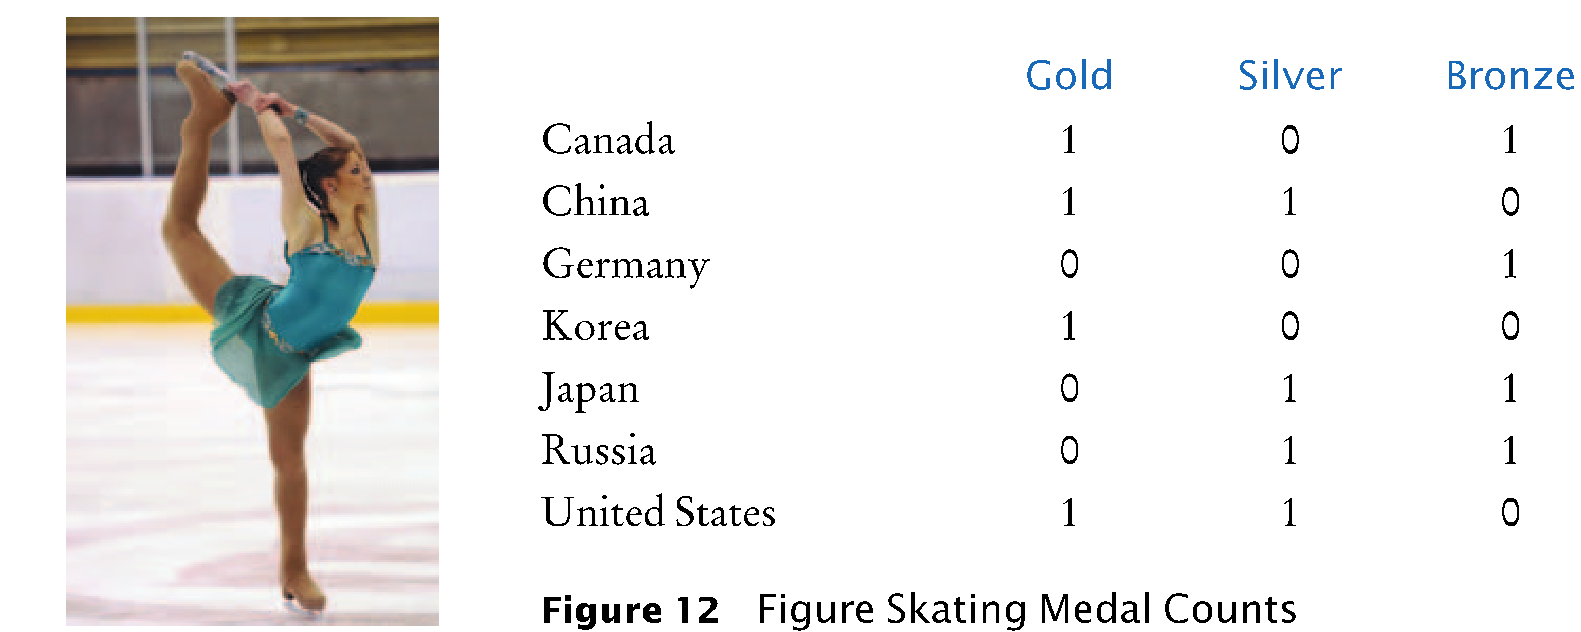
\includegraphics[width=0.83\paperwidth]{image41.png}
  \vfill
\end{frame}

% =====================================================================
%  51  Declaring Two-Dimensional Arrays
% =====================================================================
\begin{frame}[fragile]{Declaring Two-Dimensional Arrays}
  \begin{itemize}
    \item Use two `pairs' of square braces
  \end{itemize}
  \begin{columns}[T]
    \begin{column}{0.68\textwidth}
\begin{lstlisting}
final int COUNTRIES = 7;
final int MEDALS = 3;
int[][] counts = new int[COUNTRIES][MEDALS];
\end{lstlisting}
      \begin{itemize}
        \item You can also initialize the array
      \end{itemize}
      \begin{columns}[T]
        \begin{column}{0.55\linewidth}
\begin{lstlisting}[basicstyle=\ttfamily\scriptsize]
final int COUNTRIES = 7;
final int MEDALS = 3;
int[][] counts =
{
  { 1, 0, 1 },
  { 1, 1, 0 },
  { 0, 0, 1 },
  { 1, 0, 0 },
  { 0, 1, 1 },
  { 0, 1, 1 },
  { 1, 1, 0 }
};
\end{lstlisting}
        \end{column}
        \begin{column}{0.43\linewidth}
          \vskip14mm
          \callout{Note the use of two `levels' of curly braces.\ \ Each row has braces with commas separating them.}
        \end{column}
      \end{columns}
    \end{column}
    \begin{column}{0.3\textwidth}
      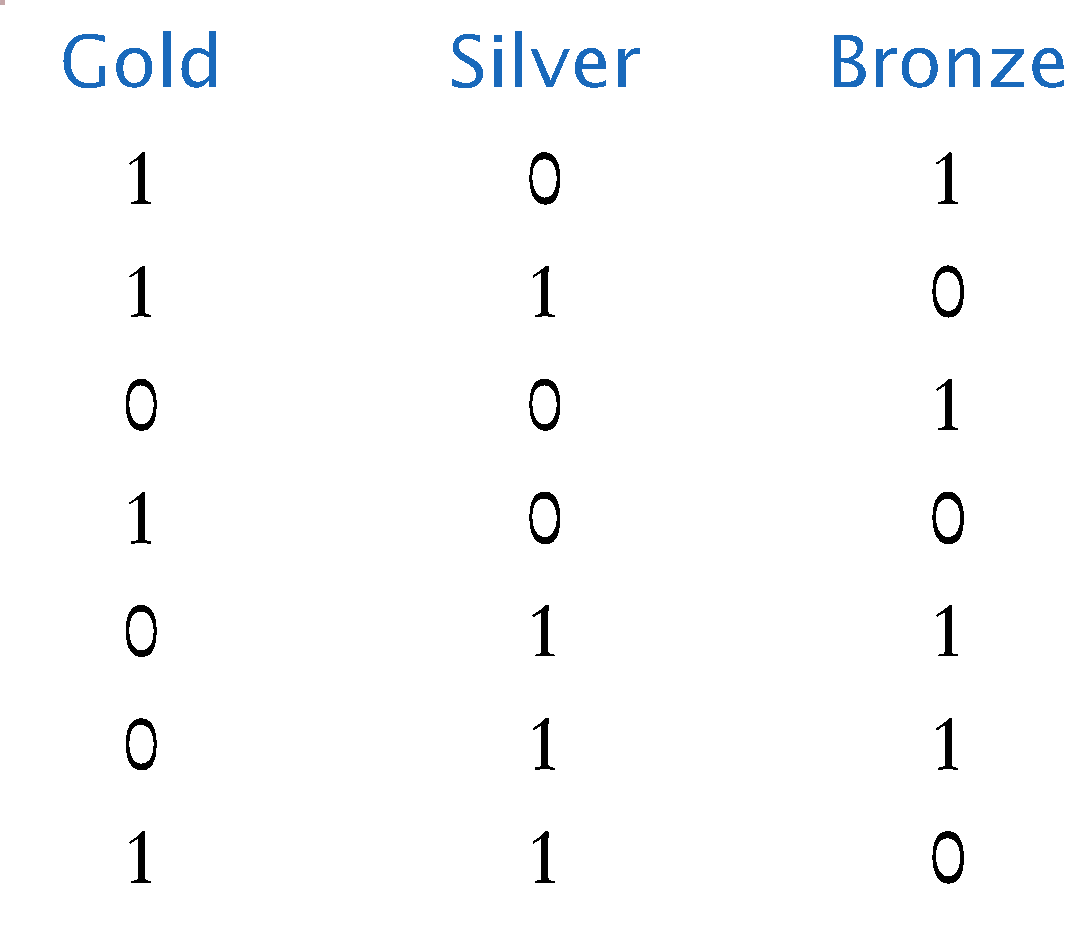
\includegraphics[width=\linewidth]{image42.png}
    \end{column}
  \end{columns}
\end{frame}

% =====================================================================
%  52  Syntax 6.3 2D Array Declaration
% =====================================================================
\begin{frame}{\syntaxtitle{6.3}{2D Array Declaration}}
  \begin{itemize}
    \item The name of the array continues to be a reference to the contents of the array
      \begin{itemize}
        \item Use new or fully initialize the array
      \end{itemize}
  \end{itemize}
  \vfill
  \centering
  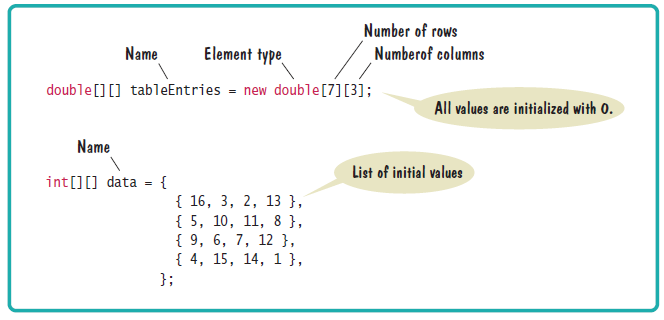
\includegraphics[width=0.86\paperwidth]{image43.png}
  \vfill
\end{frame}

% =====================================================================
%  53  Accessing Elements
% =====================================================================
\begin{frame}[fragile]{Accessing Elements}
  \begin{columns}[T]
    \begin{column}{0.62\textwidth}
      \begin{itemize}
        \item Use two index values:
      \end{itemize}
\begin{lstlisting}[linewidth=0.7\linewidth,xleftmargin=0.1\linewidth]
int value = counts[3][1];
\end{lstlisting}
      \begin{itemize}
        \item[]
          \begin{itemize}
            \item[] \hspace*{0.3\linewidth} Row then Column
          \end{itemize}
        \item To print
          \begin{itemize}
            \item Use nested for loops
            \item Outer row(\code{i}) , inner column(\code{j}) :
          \end{itemize}
      \end{itemize}
    \end{column}
    \begin{column}{0.36\textwidth}
      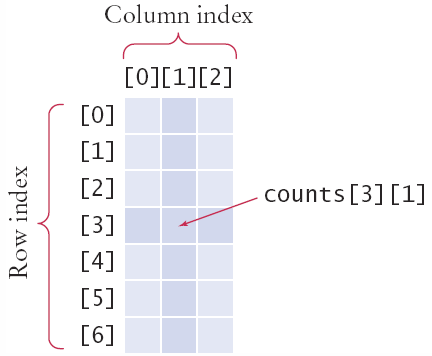
\includegraphics[width=\linewidth]{image44.png}
    \end{column}
  \end{columns}
\begin{lstlisting}
for (int i = 0; i < COUNTRIES; i++)
{
  // Process the ith row
  for (int j = 0; j < MEDALS; j++)
  {
    // Process the jth column in the ith row
    System.out.printf("%8d", counts[i][j]);
  }
  System.out.println(); // Start a new line at the end of the row
}
\end{lstlisting}
\end{frame}

% =====================================================================
%  54  Medals.java (1)
% =====================================================================
\begin{frame}[fragile]{Medals.java (1)}
  \begin{columns}[T]
    \begin{column}{0.6\textwidth}
\begin{lstlisting}[style=program]
/**
   This program prints a table of medal winner counts with row totals.
*/
public class Medals
{
   public static void main(String[] args)
   {
      final int COUNTRIES = 7;
      final int MEDALS = 3;

      String[] countries =
         {
            "Canada",
            "China",
            "Germany",
            "Korea",
            "Japan",
            "Russia",
            "United States"
         };
\end{lstlisting}
    \end{column}
    \begin{column}{0.38\textwidth}
      \vskip20mm
\begin{lstlisting}[style=program,firstnumber=21]

      int[][] counts =
         {
            { 1, 0, 1 },
            { 1, 1, 0 },
            { 0, 0, 1 },
            { 1, 0, 0 },
            { 0, 1, 1 },
            { 0, 1, 1 },
            { 1, 1, 0 }
         };
\end{lstlisting}
    \end{column}
  \end{columns}
\end{frame}

% =====================================================================
%  55  Medals.java (2)
% =====================================================================
\begin{frame}[fragile]{Medals.java (2)}
\begin{lstlisting}[style=program,firstnumber=32,basicstyle=\ttfamily\fontsize{5.9}{7}\selectfont]

      System.out.println("        Country    Gold  Silver  Bronze   Total");

      // Print countries, counts, and row totals
      for (int i = 0; i < COUNTRIES; i++)
      {
         // Process the ith row
         System.out.printf("%15s", countries[i]);

         int total = 0;

         // Print each row element and update the row total
         for (int j = 0; j < MEDALS; j++)
         {
            System.out.printf("%8d", counts[i][j]);
            total = total + counts[i][j];
         }

         // Display the row total and print a new line
         System.out.printf("%8d\n", total);
      }
   }
}
\end{lstlisting}
  \begin{tikzpicture}[remember picture,overlay]
    \node[anchor=south east,inner sep=0pt] at ([xshift=-3mm,yshift=5mm]current page.south east)
      {\programrun{0.38\paperwidth}{%
        \fontsize{5.4}{6.6}\selectfont\setlength{\tabcolsep}{1.6pt}%
        \begin{tabular}{@{}rrrrr@{}}
          Country & Gold & Silver & Bronze & Total\\
          Canada        & 1 & 0 & 1 & 2\\
          China         & 1 & 1 & 0 & 2\\
          Germany       & 0 & 0 & 1 & 1\\
          Korea         & 1 & 0 & 0 & 1\\
          Japan         & 0 & 1 & 1 & 2\\
          Russia        & 0 & 1 & 1 & 2\\
          United States & 1 & 1 & 0 & 2
        \end{tabular}}};
  \end{tikzpicture}
\end{frame}

% =====================================================================
%  56  Section: ArrayList
% =====================================================================
\section{Array Lists}
\begin{frame}[plain]
  \vfill
  \begin{center}
    {\Large\bfseries ArrayList\par}
    \vskip1mm
    {\color{titlerule}\rule{0.6\paperwidth}{1.3pt}}
  \end{center}
  \vfill
\end{frame}

% =====================================================================
%  57  Array Lists
% =====================================================================
\begin{frame}{Array Lists}
  \begin{itemize}
    \item When you write a program that collects values, you don't always know how many values you will have.
    \item In such a situation, a Java ArrayList offers two significant advantages:
      \begin{itemize}
        \item Array Lists can grow and shrink as needed.
        \item The \code{ArrayList} class supplies methods for common tasks, such as inserting and removing elements.
      \end{itemize}
  \end{itemize}
\end{frame}

% =====================================================================
%  58  Declaring and Using Array Lists
% =====================================================================
\begin{frame}[fragile]{Declaring and Using Array Lists}
  \begin{itemize}
    \item The \code{ArrayList} class is part of the \code{java.util} package
      \begin{itemize}
        \item It is a \emph{generic} class
          \begin{itemize}
            \item Designed to hold many types of objects
          \end{itemize}
        \item Provide the type of element during declaration
          \begin{itemize}
            \item Inside \code{< >} as the `type parameter'
            \item The type must be a Class
            \item Cannot be used for primitive types (\code{int}, \code{double}\ldots)
          \end{itemize}
      \end{itemize}
  \end{itemize}
  \vskip2mm
\begin{lstlisting}[linewidth=0.85\linewidth,xleftmargin=0.05\linewidth]
ArrayList<String> names = new ArrayList<String>();
\end{lstlisting}
\end{frame}

% =====================================================================
%  59  Syntax 6.4 Array Lists
% =====================================================================
\begin{frame}{\syntaxtitle{6.4}{Array Lists}}
  \begin{itemize}
    \item ArrayList provides many useful methods:
      \begin{itemize}
        \item add:\ \ add an element
        \item get: return an element
        \item remove: delete an element
        \item set:\ \ \ change an element
        \item size: current length
      \end{itemize}
  \end{itemize}
  \vfill
  \centering
  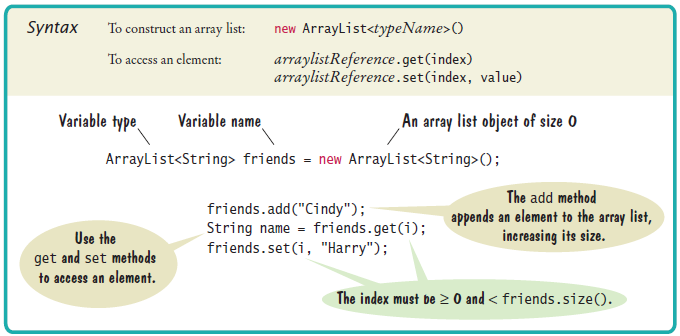
\includegraphics[width=0.78\paperwidth]{image49.png}
\end{frame}

% =====================================================================
%  60  Adding an Element with add()
% =====================================================================
\begin{frame}{Adding an Element with \texttt{add()}}
  \begin{itemize}
    \item The add method has two versions:
      \begin{itemize}
        \item Pass a new element to add to the end
          \hspace*{4mm}\colorbox{codebg}{\code{names.add("Cindy");}}
        \item Pass a location (index) and the new value to add
          \\\colorbox{codebg}{\code{names.add(1,"Cindy");}}\hspace*{6mm} Moves all other elements
      \end{itemize}
  \end{itemize}
  \vskip2mm
  \hfill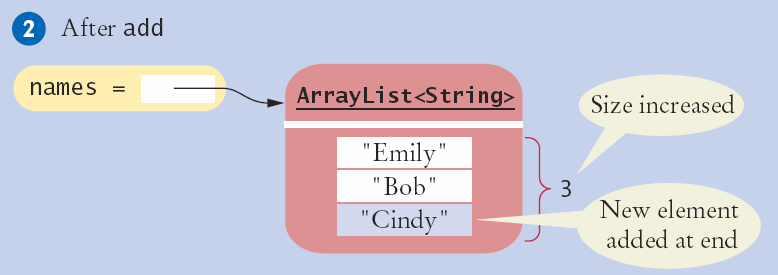
\includegraphics[width=0.6\paperwidth]{image50.png}\par
  \vskip-10mm
  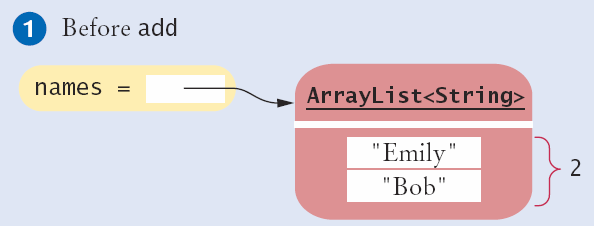
\includegraphics[width=0.48\paperwidth]{image51.png}
\end{frame}

% =====================================================================
%  61  Adding an Element in the Middle
% =====================================================================
\begin{frame}[fragile]{Adding an Element in the Middle}
  \begin{itemize}
    \item Pass a location (index) and the new value to add
      \begin{itemize}
        \item Moves all other elements
      \end{itemize}
  \end{itemize}
  \vskip2mm
  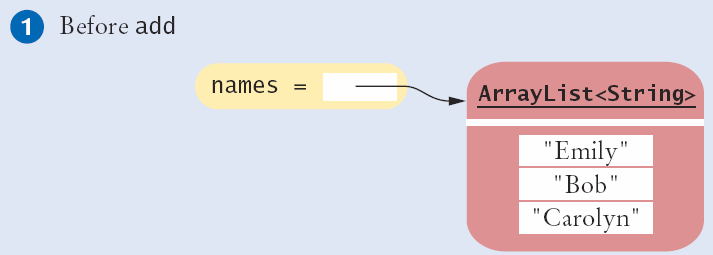
\includegraphics[width=0.6\paperwidth]{image52.png}\par
  \begin{minipage}[t]{0.38\linewidth}
    \vskip3mm
\begin{lstlisting}
names.add(1, "Ann");
\end{lstlisting}
  \end{minipage}\hfill
  \begin{minipage}[t]{0.6\linewidth}
    \vskip0pt
    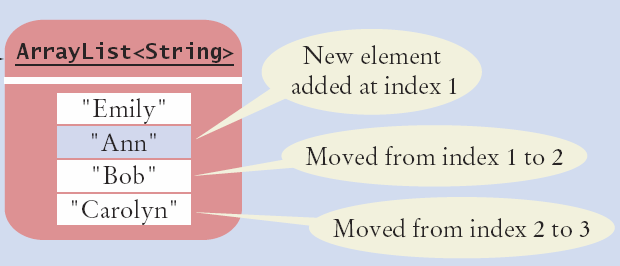
\includegraphics[width=\linewidth]{image53-cropped.png}
  \end{minipage}
\end{frame}

% =====================================================================
%  62  Removing an Element
% =====================================================================
\begin{frame}[fragile]{Removing an Element}
  \begin{itemize}
    \item Pass a location (index) to be removed
      \begin{itemize}
        \item Moves all other elements
      \end{itemize}
  \end{itemize}
  \vskip2mm
  \hspace*{0.08\paperwidth}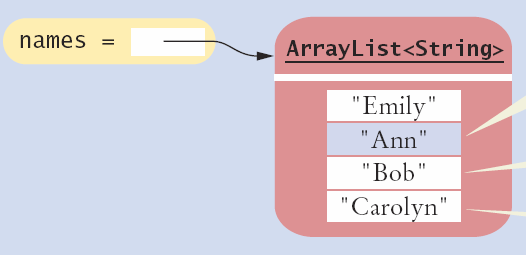
\includegraphics[width=0.48\paperwidth]{image54.png}\par
  \begin{minipage}[t]{0.32\linewidth}
    \vskip3mm
\begin{lstlisting}
names.remove(1);
\end{lstlisting}
  \end{minipage}\hfill
  \begin{minipage}[t]{0.62\linewidth}
    \vskip0pt
    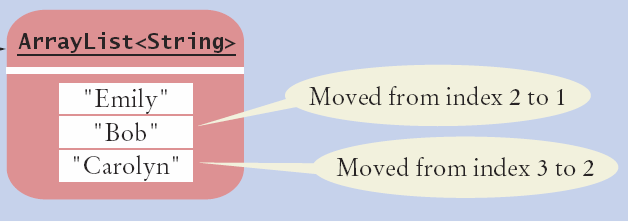
\includegraphics[width=\linewidth]{image55.png}
  \end{minipage}
\end{frame}

% =====================================================================
%  63  Using Loops with Array Lists
% =====================================================================
\begin{frame}[fragile]{Using Loops with Array Lists}
  \begin{itemize}
    \item You can use the enhanced for loop with Array Lists:
  \end{itemize}
\begin{lstlisting}[linewidth=0.6\linewidth,xleftmargin=0.1\linewidth]
ArrayList<String> names = . . . ;
for (String name : names)
{
  System.out.println(name);
}
\end{lstlisting}
  \vskip2mm
  \begin{itemize}
    \item Or ordinary loops:
  \end{itemize}
\begin{lstlisting}[linewidth=0.66\linewidth,xleftmargin=0.1\linewidth]
ArrayList<String> names = . . . ;
for (int i = 0; i < names.size(); i++)
{
  String name = names.get(i);
  System.out.println(name);
}
\end{lstlisting}
\end{frame}

% =====================================================================
%  64  Working with Array Lists
% =====================================================================
\begin{frame}{Working with Array Lists}
  \vfill
  \centering
  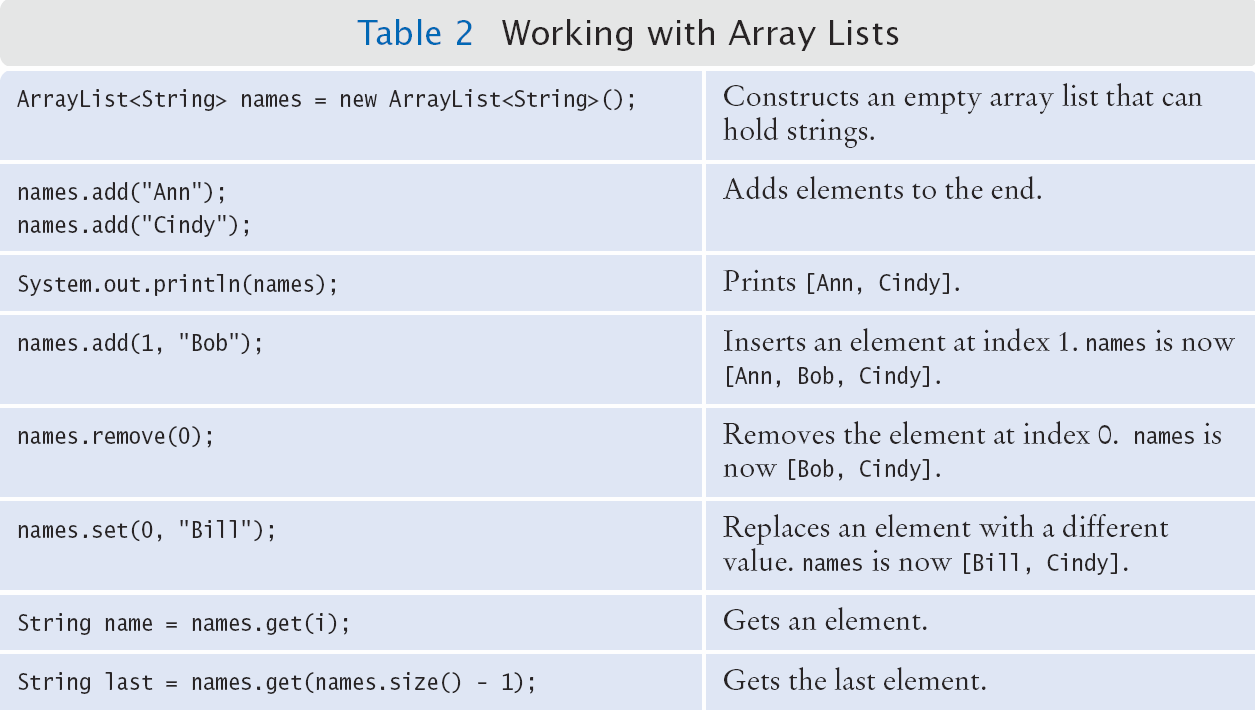
\includegraphics[width=\linewidth]{image56.png}
  \vfill
\end{frame}

% =====================================================================
%  65  Copying an ArrayList
% =====================================================================
\begin{frame}[fragile]{Copying an \texttt{ArrayList}}
  \begin{itemize}
    \item Remember that \code{ArrayList} variables hold a reference to an \code{ArrayList} (just like arrays)
  \end{itemize}
  \begin{columns}[T]
    \begin{column}{0.5\textwidth}
      \begin{itemize}
        \item Copying a reference:
      \end{itemize}
\begin{lstlisting}
ArrayList<String> friends = names;
friends.add("Harry");
\end{lstlisting}
    \end{column}
    \begin{column}{0.48\textwidth}
      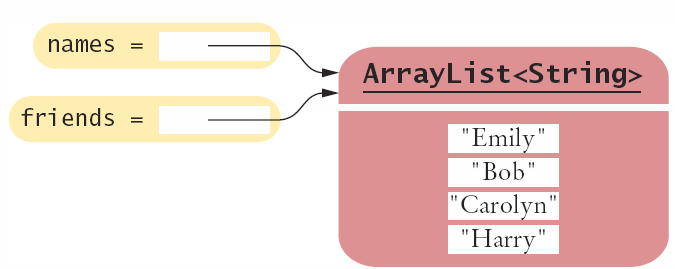
\includegraphics[width=\linewidth]{image57.png}
    \end{column}
  \end{columns}
  \vskip2mm
  \begin{itemize}
    \item To make a copy, pass the reference of the original \code{ArrayList} to the constructor of the new one:
  \end{itemize}
  \hfill\ptag{reference $\downarrow$}\hspace*{0.1\linewidth}
\begin{lstlisting}
ArrayList<String> newNames = new ArrayList<String>(names);
\end{lstlisting}
\end{frame}

% =====================================================================
%  66  Array Lists and Methods
% =====================================================================
\begin{frame}[fragile]{Array Lists and Methods}
  \begin{itemize}
    \item Like arrays, Array Lists can be method parameter variables and return values
    \item Here is an example: a method that receives a list of \code{String}s and returns the reversed list
  \end{itemize}
  \hfill\ptag{reference $\downarrow$}\hspace*{0.05\linewidth}
\begin{lstlisting}[basicstyle=\ttfamily\scriptsize]
public static ArrayList<String> reverse(ArrayList<String> names)
{
  // Allocate a list to hold the method result
  ArrayList<String> result = new ArrayList<String>();
  // Traverse the names list in reverse order (last to first)
  for (int i = names.size() - 1; i >= 0; i--)
  {
    // Add each name to the result
    result.add(names.get(i));
  }
  return result;
}
\end{lstlisting}
\end{frame}

% =====================================================================
%  67  Wrappers and Auto-boxing (1)
% =====================================================================
\begin{frame}[fragile]{Wrappers and Auto-boxing}
  \begin{columns}[T]
    \begin{column}{0.6\textwidth}
      \begin{itemize}
        \item Java provides \emph{wrapper} classes for primitive types
          \begin{itemize}
            \item Conversions are automatic using \textbf{\emph{auto-boxing}}
              \begin{itemize}
                \item Primitive to \code{wrapper} Class
              \end{itemize}
          \end{itemize}
      \end{itemize}
\begin{lstlisting}[linewidth=0.75\linewidth,xleftmargin=0.2\linewidth]
double x = 29.95;
Double wrapper;
wrapper = x;  // boxing
\end{lstlisting}
      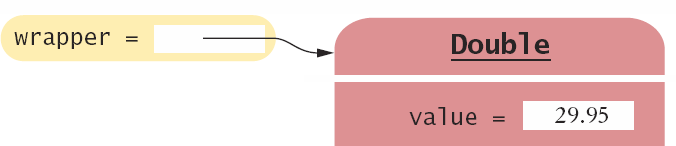
\includegraphics[width=0.85\linewidth]{image59.png}
      \begin{itemize}
        \item[]
          \begin{itemize}
            \item[]
              \begin{itemize}
                \item \code{wrapper} Class to primitive
              \end{itemize}
          \end{itemize}
      \end{itemize}
\begin{lstlisting}[linewidth=0.75\linewidth,xleftmargin=0.2\linewidth]
double x;
Double wrapper = 29.95;
x = wrapper;  // unboxing
\end{lstlisting}
    \end{column}
    \begin{column}{0.38\textwidth}
      \vskip4mm
      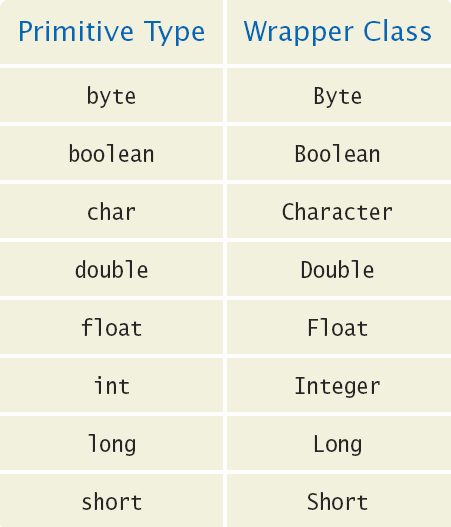
\includegraphics[width=\linewidth]{image58.png}
    \end{column}
  \end{columns}
\end{frame}

% =====================================================================
%  68  Wrappers and Auto-boxing (2)
% =====================================================================
\begin{frame}[fragile]{Wrappers and Auto-boxing}
  \begin{itemize}
    \item You cannot use primitive types in an \code{ArrayList}, but you can use their wrapper classes
      \begin{itemize}
        \item Depend on auto-boxing for conversion
      \end{itemize}
    \item Declare the \code{ArrayList} with wrapper classes for primitive types
      \begin{itemize}
        \item Use \code{ArrayList<Double>}
          \begin{itemize}
            \item Add primitive double variables
            \item Or \code{double} values
          \end{itemize}
      \end{itemize}
  \end{itemize}
\begin{lstlisting}[linewidth=0.82\linewidth,xleftmargin=0.12\linewidth]
double x = 19.95;
ArrayList<Double> values = new ArrayList<Double>();
values.add(29.95);          // boxing
values.add(x);              // boxing
double y = values.get(0);   // unboxing
\end{lstlisting}
\end{frame}

% =====================================================================
%  69  ArrayList Algorithms
% =====================================================================
\begin{frame}[fragile]{\texttt{ArrayList} Algorithms}
  \begin{columns}[T]
    \begin{column}{0.36\textwidth}
      \begin{itemize}
        \item Converting from Array to \code{ArrayList} requires changing:
          \begin{itemize}
            \item index usage: \code{[i]}
            \item \code{values.length}
          \end{itemize}
        \item To
          \begin{itemize}
            \item methods: \code{get()}
            \item \code{values.size()}
          \end{itemize}
      \end{itemize}
    \end{column}
    \begin{column}{0.62\textwidth}
\begin{lstlisting}
double largest = values[0];
for (int i = 1; i < values.length; i++)
{
  if (values[i] > largest)
  {
    largest = values[i];
  }
}
\end{lstlisting}
      \vskip2mm
\begin{lstlisting}
double largest = values.get(0);
for (int i = 1; i < values.size(); i++)
{
  if (values.get(i) > largest)
  {
    largest = values.get(i);
  }
}
\end{lstlisting}
    \end{column}
  \end{columns}
\end{frame}

% =====================================================================
%  70  Choosing Arrays or Array Lists
% =====================================================================
\begin{frame}{Choosing Arrays or Array Lists}
  \begin{itemize}
    \item Use an Array if:
      \begin{itemize}
        \item The size of the array never changes
        \item You have a long list of primitive values
          \begin{itemize}
            \item For efficiency reasons
          \end{itemize}
        \item Your instructor wants you to
      \end{itemize}
    \item Use an Array List:
      \begin{itemize}
        \item For just about all other cases
        \item Especially if you have an unknown number of input values
      \end{itemize}
  \end{itemize}
\end{frame}

% =====================================================================
%  71  Array and Array List Operations
% =====================================================================
\begin{frame}{Array and Array List Operations}
  \vfill
  \centering
  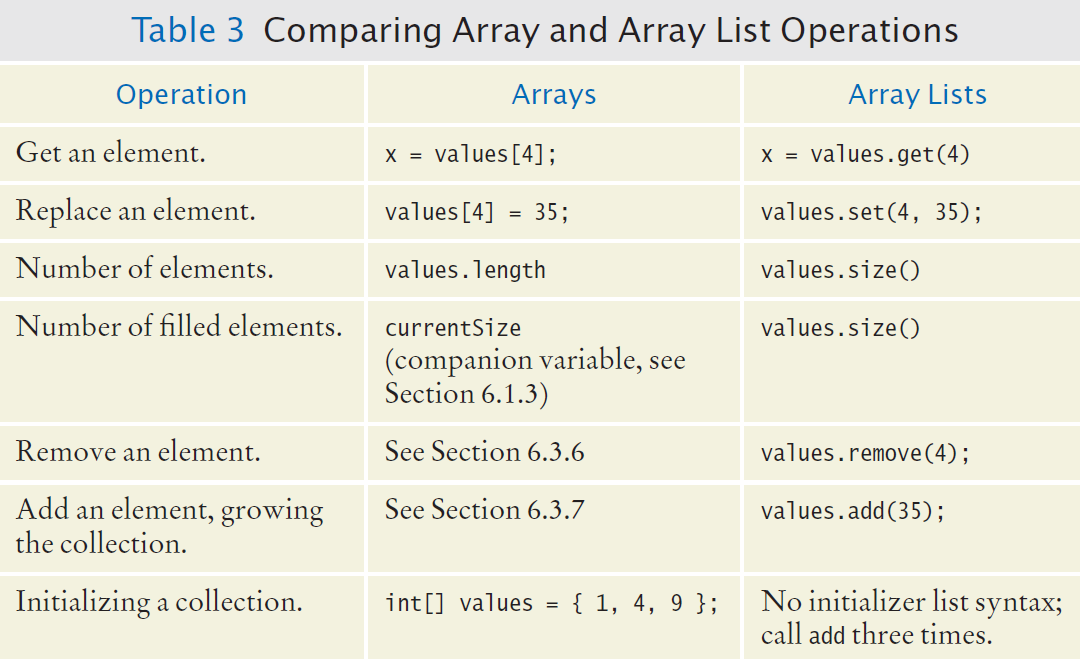
\includegraphics[width=\linewidth,height=0.74\paperheight,keepaspectratio]{image60.png}
  \vfill
\end{frame}

% =====================================================================
%  72--73  Self Checks 6.39--6.40   (hidden in the original)
% =====================================================================
\begin{frame}<\hiddenslides>[fragile]{Self Check 6.39}
  Declare an array list \code{primes} of integers that contains the first five prime
  numbers (2, 3, 5, 7, and 11).
  \vskip3mm
  \answer
\begin{lstlisting}[linewidth=0.6\linewidth,xleftmargin=8mm,backgroundcolor={},frame=none]
ArrayList<Integer> primes =
  new ArrayList<Integer>();
primes.add(2);
primes.add(3);
primes.add(5);
primes.add(7);
primes.add(11);
\end{lstlisting}
\end{frame}

\begin{frame}<\hiddenslides>[fragile]{Self Check 6.40}
  Given the array list \code{primes} declared in Self Check 39, write a loop to print its
  elements in reverse order, starting with the last element.
  \vskip3mm
  \answer
\begin{lstlisting}[linewidth=0.7\linewidth,xleftmargin=8mm,backgroundcolor={},frame=none]
for (int i = primes.size() - 1; i >= 0; i--)
{
   System.out.println(primes.get(i));
}
\end{lstlisting}
\end{frame}

% =====================================================================
%  74  Common Error -- Length versus Size
% =====================================================================
\begin{frame}{Common Error}
  \begin{itemize}
    \item Length versus Size
      \begin{itemize}
        \item Unfortunately, the Java syntax for determining the number of elements in an
              array, an \code{ArrayList}, and a \code{String} is not consistent.
        \item It is a common error to confuse these. You just have to remember the correct
              syntax for each data type.
      \end{itemize}
  \end{itemize}
  \vfill
  \centering
  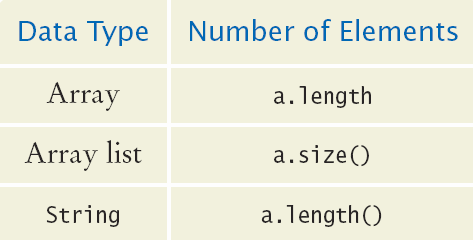
\includegraphics[width=0.52\paperwidth]{image61.png}
  \vfill
\end{frame}

\end{document}
